\section{Classification}
\label{sec:exp-clf}
    \subsection{Overview}
    \label{subsec:exp-clf-overview}
        \newcommand{\optnode}[5]{
    % supernode id, find content, assume content, found content, position 
    \node (#1-find) [smallamber,minimum height=0.1cm ,text width=1.6cm,minimum width = 2cm #5] {\specialcell{#2}};
    \node (#1-assume) [smalldarkbyzantium,minimum height=0.1cm, text width=1.6cm, minimum width = 2cm, below=0.15cm of #1-find] {\specialcell{#3}};
    \node (#1-found) [smallazure,minimum height=0.1cm, text width=1.6cm, minimum width = 2cm, below=0.15cm of #1-assume] {\specialcell{#4}};
    \begin{pgfonlayer}{background}
        \node(#1)[bigblush] [fit = (#1-find) (#1-found)] {};
    \end{pgfonlayer}
}
\def\dist{0.3cm}
\begin{tikzfig}{fig:exp-clf-overview-opt}{Optimisation and iteration of pre-classification pipeline.}{\tiny}
    
    \optnode{feats}{choose features}{balance classes\\normalise audio\\training labels\\classifier params}{normalise features\\testing label}{}
    \optnode{balance}{balance classes}{normalise audio\\training labels\\classifier params}{normalise features\\testing label\\chosen features}{, right=\dist of feats-find}
    \optnode{normaud}{normalise audio}{training labels\\classifier params}{normalise features\\testing label\\chosen features\\balance classes}{, right=\dist of balance-find}
    \optnode{labels}{choose train labels}{classifier params}{normalise features\\testing label\\chosen features\\balance classes\\normalise audio}{, right=\dist of normaud-find}
    \optnode{clf}{classifier params}{none}{normalise features\\testing label\\chosen features\\balance classes\\normalise audio\\chosen train labels}{, right=\dist of labels-find}
    \optnode{done}{none}{none}{normalise features\\testing label\\chosen features\\balance classes\\normalise audio\\chosen train labels\\classifier params}{, right=\dist of clf-find}
    
    \optnode{key}{optimising}{assumed}{chosen/estimated}{, left=3cm of balance-find}

    \draw[arrow](feats)--(balance);
    \draw[arrow](balance)--(normaud);
    \draw[arrow](normaud)--(labels);
    \draw[arrow](labels)--(clf);
    \draw[arrow](clf)--(done);
    \draw [arrow] (done-found.east) -| (12.85,-3.37) |- (-1.4,-3.37)  node[near end,above]{iterate}-| (-1.4,-2) |- (feats-assume.west);

    
\end{tikzfig}
        In this section, parameters that alter the training set of data and those which affect the training process itself will be experimentally optimised to increase classification performance. An exhaustive grid search for the parameters discussed here would require training and testing of each classifier hundreds of thousands of times, taking tens of thousands of days of computing time. Instead, an sequential approach will be taken, depicted in figure \ref{fig:exp-clf-overview-opt}. 
    
        For each stage, one parameter/set of parameters is locally optimised whilst making initial assumptions about the others. This approach reduces the required number of train/test cycles by several orders of magnitude, making optimisation of this pipeline computationally feasible. Cross-validation is used for every stage in the pipeline; the model with the highest performing hyperparameter combination is chosen and then tested on `unseen' data, results of which are presented in table \ref{sec:appdx-xvalres}. Model selection decisions will \textit{not} be influenced by test results on unseen data for reasons discussed in section \ref{subsec:exp-clf-xval}. This section is strongly linked with sections \ref{sec:pl-data} to \ref{sec:pl-clf}, which detail the mathematics and implementation specifics of the procedures highlighted here.
        
        Performance will be evaluated over each of the chosen classifiers using the metrics $F_{1}$ score, area under the receiver-operator curve (AUC-ROC), area under the precision-recall curve (AUC-PR), true positive rate (TPR), and the true negative (TNR) rate. These metrics have been chosen as they represent important classifier characteristics in a compact form, convenient for comparing many results. More details regarding metrics can be found in section \ref{sec:pl-test}. 

        % limitations of this approach, initial parameter selection will `steer` it down a specific route which iteration wont solve but only possible approach, could be overcome by randomly seeding initial assumptions then iterating through those pipelines but still too much computation required
      
     
    \subsection{Classifier Selection}
    \label{subsec:exp-clf-select}
        Of the set of implemented classifiers listed in the first row of appendix \ref{sec:appdx-xvalres}, a subset is chosen to further develop for this mosquito detection pipeline. Initial experiments are ran with the assumptions listed in section \ref{subsec:exp-clf-ass}. As a simple initial test, the data is randomly divided into two equal sets and each classifier is tested.
        
        Results are shown in the first row of appendix \ref{sec:appdx-xvalres}. The decision tree classifier performs poorly relative to other classifiers, but is significantly improved by using many together, i.e. a random forest classifier, which substantially reduces overfit through random subsampling of features; for this reason the decision tree is dropped in favour of the random forest. The lowest scoring predictor is the Gaussian mixture model classifier; this is discarded in favour of the naive Bayes classifier which shares some similarities, but at reduced complexity and increased speed and performance. The $k$-Nearest-Neighbours algorithm has a somewhat satisfactory $F_1$ score, but is severely unbalanced in terms of class predictions and suffers from slow classification time, so will not be used further. Testing an SVM with three kernels reveals that both the linear and polynomial kernels are slow and perform worse than the radial basis function kernel; this kernel with the SVM produces the best results so is selected for further use.

        Deep learning methods, such as artificial neural networks (ANNs), convolutional neural networks (CNNs) and multi-layer perceptrons (MLPs), are not considered for use in this project. These techniques, although implementable in MozzPy, behave fundamentally differently to traditional classifiers. Instead of `hand-crafting' features, features are learned from the raw input which is often a frequency representation of the signal. This approach requires a different pipeline to that which is explored in this project; hence, deep learning techniques are explored parallel to this research by \textcite{Kiskin} as part of the HumBug team.
        
        
        % red for bad green for blue in table
        
        % A naive Bayes classifier is chosen as it. cant crossval as some classifiers take too much time, fine to test on held out data as only using it to select classifiers not tune them
        % [naive bayes, gaussian mixture model, knn, svm, random forest, decision tree]
        % kNN - too long, lazy classifier computed at runtime - using 8 cores took 3 hours with results as good as rf
        % naive bayes - simple, easy, no params, likely weak but very fast and good for testing, will optimise along pipeline
        % gmm - very similar but worse performance than bayes, more params, slower %https://stats.stackexchange.com/questions/105140/gaussian-naive-bayes-really-equivalent-to-gmm-with-diagonal-covariance-matrices
        % gps - memory errors, not the best for audio classification or classification in general - find citation
        % svm - rbf great performance, other kernels struggle to do as good
       
    \subsection{Cross Validation}
    \label{subsec:exp-clf-xval}
        In tuning a model for mosquito detection, it is imperative that the predictive model is generalisable to unseen data. Given the set of Culex. \textit{q.} data, it would be possible to train a classifier over the whole set of data; this would give a near-perfect score if tested on the same data but obviously gives no information regarding generalisation ability of the model. By splitting the data into a testing and training set, a classifier can be trained on one set of data and tested on another. As the hyperparameters of the pipeline are tweaked to optimise classifier performance over the test set, information from the test set `leaks' into the model selection process, leading to overfit and a no-longer generalisable model. A further split of the training set can be made, giving a validation set. With this, the model is trained, evaluated and optimised over these two sets, then tested on the `unseen' test set. Results of the tests can then be generalised to any unseen data; this is called `hold-out' validation. In practise, this method is often only used when simplicity of implementation and low computational complexity are favoured because information in the training set is not utilised fully, resulting in a bias towards underestimating performance.
     
        Instead, the preferred method is to split data is split into two then perform $k$-fold cross-validation over the training set, removing the need for a validation set. By including all the samples in both training and testing, bias is reduced. Generally, a higher choice of $k$ reduces the bias as the contents of the training folds begin to approach that of the total dataset. This comes at the expense of increasing both the computational load and the variability of the results over each fold due to the smaller test set sizes being more sensitive to outliers. The Culex \textit{q.} data, split into windows of length \SI{0.0125}{\second} and step \SI{0.01}{\second}, contains $299095$ samples. With this medium to large sized data set, the choice of $k$ becomes less significant \cite{Kohavi1995}. 
        
        Another method, `leave one out' cross-validation, is the extreme of $k$-fold validation with $k$ equal to the number of samples. This method produces the theoretically lowest bias at the cost of very high variance due to predictions being made over one sample at a time as well as extreme computational load, hence it will not be used for this pipeline.

        Initially, the data will be split into two equal, randomly sampled sets. An equal split provides a large enough set of data to test on and give a sufficient idea of the models validity and generalisability to unseen data. For reasonable performance whilst utilising the benefits of $k$-fold cross validation, $k=5$ is used with the addition stratification to preserve original mosquito/no-mosquito class proportions. Cross-validated parameters are summarised in appendix \ref{sec:appdx-xvalres} and details of algorithm implementation and methodology are provided in section \ref{subsec:pl-test-xval}. Time dependency of the data will be ignored in this section and each sample will be treated as independently and identically distributed; this is a weak assumption but greatly simplifies the optimisation process. More sophisticated cross-validation techniques can be employed as outlined in the research by \textcite{Yang2001}; however, time-dependency will be exploited during post-processing in section \ref{sec:exp-postproc}.
        
        % https://www.analyticsvidhya.com/blog/2015/11/improve-model-performance-cross-validation-in-python-r/
        
    
        
        % http://scikit-learn.org/stable/modules/cross_validation.html v good basic details
     
         
  
    
        % model selection for this pipeline will take place in structured way
        % inner-cv loop will select parametrs for each stage defined in fig 5. then validation score will be calculated on held out dataset for indication of how well its doing
        % no decisions made based on validation score, keeps bias at a minimum
        % https://www.ncbi.nlm.nih.gov/pmc/articles/PMC1397873/ - paper on cv
        % ideally would do over whole parameter space
        % many python implementations of CV exist already but only for standard problems such as feature selection (not feature parameter tuning) and classifier parameter selection
        % data must be i.i.d - time series so not really?
        % each sample treated individually
        % LOO CV
        % more folds decrease variance increase bias
        % 50/50 good estimate of performance
        %   large dataset good for estimating generalisation error for resultant classifier
        % this way get a decent model with low overfit/
        % data driven daaptation of classifier
        
    \subsection{Known Parameters}
    \label{subsec:exp-clf-known}  
        \subsubsection{Feature Normalisation}
        \label{subsubsec:exp-clf-known-featnorm}
            Feature normalisation, or \textit{whitening}, is done with reuse of constants for reasons discussed in section \ref{subsec:pl-data-software}. The impact of normalisation depends on the nature of the classifier being used and how similarity/distance is defined. For a random forest classifier, decisions whether to split a node are based on the information/entropy of the feature (discussed further in section \ref{subsec:pl-clf-sup}), a criteria that is invariant to monotonic transforms such as feature scaling \cite{Hastie2009}, so normalisation will not be applied for the random forest.
            
            SVM performance, in comparison, is dependent on feature scaling. By not scaling, a feature with larger magnitudes may be assigned a higher importance than one with lower magnitudes. The RBF kernel uses the squared Euclidian distance as a measure of similarity so normalisation is essential for this classifier. Naive Bayes, by design, performs feature scaling when normalising by the evidence, detailed in section \ref{subsec:pl-clf-sup}.
            
            These conclusions have been confirmed in brief trials where both the random forest and naive Bayes classifiers were unaffected by feature normalisation, and the SVM without normalisation was $\sim10$ times slower to train with resultant $F_{1}$ scores reduced by at least $0.2$.
    
            %[http://stats.stackexchange.com/questions/57010/is-it-essential-to-do-normalization-for-svm-and-random-forest]
            
        \subsubsection{Feature Parameters}
        \label{subsubsec:exp-clf-known-featparam}
            Each feature is generated using a number of parameters. To cross-validate over a grid of possible parameters would be impractical. Instead, defaults will be used, defined in section \ref{subsec:pl-feats-software}. The only parameters varied will be \code{'winlen'} and \code{'winstep'} as this is universal across all features and feasible to optimise.
        
        \subsubsection{Testing Labels}
        \label{subsubsec:exp-clf-known-tstlbls}
            \begin{wrapfigure}{r}{0.3\textwidth}
                \centering
                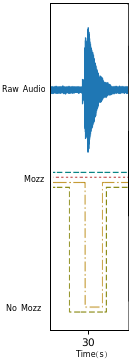
\includegraphics[width=0.2\textwidth]{label_example}
                \caption{An example of noise where there is $50/50$ disagreement between labellers.}
                \label{fig:exp-clf-known-tstlbls-exmp}
            \end{wrapfigure}
            All the possible training/testing pairs are shown in tables \ref{tbl:exp-clf-known-tstlbls-bintbl} and \ref{tbl:exp-clf-known-tstlbls-multitbl}; details of which are given in section \ref{subsec:pl-data-software}. Although there are $24$ aggregation policies in total, it would be incorrect to optimise the pipeline by varying the test labels as this introduces a bias of being able to choose how correct a set of predictions are. Instead, a universal test label should be chosen that reflects the actual data as close as possible. For these experiments, `05\_notmozz' will be selected, representing a majority vote where at least 3/4 of votes are needed for a positive label. This is based on inspection of many areas of the recordings in which there is irregular noise, such as talking over the sound of a mosquito. Often, two people will class this as positive and two negative, as shown in figure \ref{fig:exp-clf-known-tstlbls-exmp}. In terms of classification, it is desirable to treat this as a negative example to prevent voices being classed as positive; hence, a majority voting policy will be employed.

            \begin{table}
                \scriptsize
                \singlespacing
                \centering
                \subfloat[][Binary Labelling Policies]{
                    \begin{tabular}{ |l|l|c| } 
                        \hline
                        Train Label & Test Label & Use\\
                        \hline
                        `0\_5\_notmozz'&`0\_5\_notmozz'& \checkmark \\
                        `0\_5\_notmozz'&`0\_5\_ismozz'& \xmark\\
                        `0\_5\_notmozz'&`sensitive'& \xmark\\
                        `0\_5\_ismozz'&`0\_5\_ismozz'& \xmark \\
                        `0\_5\_ismozz'&`0\_5\_notmozz'& \checkmark\\
                        `0\_5\_ismozz'&`sensitive'& \xmark\\
                        `sensitive'&`sensitive'& \xmark\\
                        `sensitive'&`0\_5\_notmozz'& \checkmark \\
                        `sensitive'&`0\_5\_ismozz'& \xmark\\
                        `conf'&`0\_5\_notmozz'& \checkmark \\
                        `conf'&`0\_5\_ismozz'& \xmark\\
                        `conf'&`sensitive'& \xmark\\
                        `0\_5\_ignore`&`0\_5\_notmozz'& \checkmark \\
                        `0\_5\_ignore`&`0\_5\_ismozz'& \xmark\\
                        `0\_5\_ignore`&`sensitive'& \xmark\\
                        \hline
                    \end{tabular}
                    % \caption{Training and testing label pairing for binary labels.}
                    \label{tbl:exp-clf-known-tstlbls-bintbl}
                }
                \qquad
                \subfloat[][Multi-class Labeling Policies.]{
                    \begin{tabular}{ |l|l|l|c| } 
                        \hline
                        Train Label & Test Label & Uncertain Votes & Use\\
                        \hline
                        `multiclass'&`0\_5\_notmozz'& `ismozz' &\checkmark \\
                        `multiclass'&`0\_5\_ismozz'&`ismozz'& \xmark\\
                        `multiclass'&`sensitive' & `ismozz' & \xmark\\
                        `multiclass'&`0\_5\_notmozz' & `notmozz' &  \checkmark \\
                        `multiclass'&`0\_5\_ismozz'& `notmozz' & \xmark\\
                        `multiclass'&`sensitive'& `notmozz' & \xmark\\
                        `multiclass'&`0\_5\_notmozz'& `reject` &  \checkmark \\
                        `multiclass'&`0\_5\_ismozz'& `reject` & \xmark\\
                        `multiclass'&`sensitive'& `reject` & \xmark\\
                        \hline
                    \end{tabular}
                    % \caption{Training and testing label pairing for multi-class labels.}
                    \label{tbl:exp-clf-known-tstlbls-multitbl}
                }
                \caption{All possible training and testing label pairs.}
                \label{tbl:exp-clf-known-tstlbls-tbls}
            \end{table}
            
            % \begin{wraptable}{r}{0.6\textwidth}
            %     \scriptsize
            %     \singlespacing
            %     \centering
                    
            % \end{wraptable}
            
            
    \subsection{Parameter Assumptions}
    \label{subsec:exp-clf-ass}
        \subsubsection{Class Balancing}
        \label{subsubsec:exp-clf-ass-bal}
            Firstly, classes of the training data are balanced to contain the same number of samples in each class. For the Culex \textit{q.} dataset, after splitting the data into a training and test set and using the `conf' label aggregation policy (explained in section \ref{subsec:pl-data-software}), the training data begins with $80024$ and $24695$ samples for classes $0$ and $1$ respectively; both classes are balanced to contain $24695$ samples. Initial experiments have shown this is a sufficient sample size and often leads to better performance and dramatically faster classification times; however, more thorough experimentation will be carried out later in this section to assure this.
    
        \subsubsection{Audio Normalisation}
        \label{subsubsec:exp-clf-ass-aud}
            The Culex \textit{q.} data set was recorded using the same device in the same location for each of the 57 recordings, therefore mosquitoes flying into and out of the microphone range will have consistent volumes. Some sections of the recordings contain highly irregular noise that is considerably louder than the mosquitoes; an example noisy signal is shown in figure \ref{fig:exp-clf-audio-noisy} where the first thirty seconds contain human voices.
            \begin{figure}[ht]
                \centering
                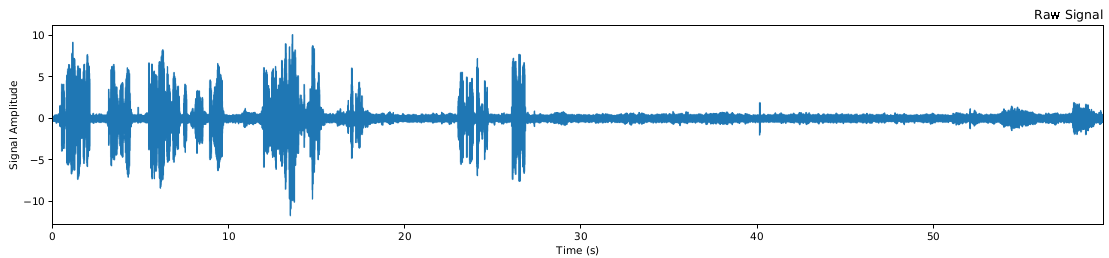
\includegraphics[width=\textwidth]{raw_with_noise}
                \caption{An example of a particularly noisy signal from the Culex. recordings where people are talking in the vicinity of the microphone.}
                \label{fig:exp-clf-audio-noisy}
            \end{figure}
            Normalising on a signal-by-signal basis can be considered bad practise for many audio-based machine learning problems due to the time-dependency of the signal, as its using information that is `from the future' for classification, leading to unpredictable consequences. However, this is acceptable in some cases in which the classifier will be used on many samples at a time rather than on a live, sample-by-sample, basis. These acceptable situations include an automated tagging system, a logger with a buffer or swarm tracking; these use cases are detailed in section \ref{subsec:bg-intro-resinterests}. For on-line applications such as a solar lamp or smartphone, there is scope for use of more sophisticated algorithms to achieve normalisation such as Automatic Gain Control (AGC), which has been shown to improve robustness and performance of speech recognition with deep neural networks \cite{Prabhavalkar2015}. However, this will be left for further research due to the complexities of implementation. No audio normalisation will be assumed at first, then the best performing combination of \code{'unit-variance'} and \code{'zero-mean'} transforms will be determined experimentally. Regarding the on-line case, where normalising signal-by-signal is incorrect, it will be assumed that a similar level performance could be achieved using more sophisticated algorithms, should normalisation in this way provide better performance than no normalisation.

        \subsubsection{Training Labels}
        \label{subsubsec:exp-clf-ass-trnlabel}
            \begin{wraptable}{r}{0.4\textwidth}
                \scriptsize
                \singlespacing
                \centering
                    \begin{tabular}{ |c|c|c|c| } 
                        \hline
                        \specialcell{No.\\ Disagreements} & 0 & 1 & 2 \\ 
                        \hline
                        \specialcell{Percentage of \\All Labels} & 77.7\% & 16.2\% & 6.04\% \\ 
                        \hline
                    \end{tabular}
                \caption{Disagreement between four people labelling the same data-set.}
                \label{fig:exp-clf-ass-label-agree}
            \end{wraptable}
            Analysis of the given labels, shown in table \ref{fig:exp-clf-ass-label-agree}, emphasises the difficulty of this problem. Of the four people labelling the data, there is only complete agreement $77\%$ of the time, the rest of the time there is at least one person who disagrees with the others. Without knowing the details of each persons labelling methodology, a uniform prior must be applied to assign them equal importance for classification use. Therefore, it can be reasoned that it is most appropriate to take a consensus vote to use information from all sets of labels. 
            
            As discussed in section \ref{subsec:pl-data-software}, there are six methods to create a binary consensus label. The \code{'conf'} label aggregation policy will be assumed initially because it is the least likely to contain miss-labelled samples; for a sample to be miss-labelled all four people must label incorrectly. 
            
        \subsubsection{Classifier Hyperparameters}
        \label{subsubsec:exp-clf-ass-param}
            Classifiers have internal parameters that determine certain aspects of their behaviour; a more in depth breakdown is given in section \ref{subsec:pl-clf-sup}. An intuition derived from the data and experiments on the data provide a basis for determining these parameters. At this stage, there is minimal intuition developed so parameters will be left at the default settings, with the exception of the \code{'n\_estimators'} parameter that defines the number of decision trees that make up the random forest classifier. The default value of $10$ trees is only adequate for very small sets of data, a value of $150$ trees will instead be assumed based on the research by \textcite{Oshiro2012a}. Overfitting is not a concern as this \textit{rarely} occurs with a random forest \cite{Breiman2001}.
        
    \subsection{Optimisation}
    \label{subsec:exp-clf-opt}
    
        \subsubsection{Feature Selection}
        \label{subsubsec:exp-clf-opt-featsel}
            Feature design and selection, as detailed in sections \ref{sec:pl-feats} and \ref{sec:pl-featpreproc}, are crucial to any machine learning problem using traditional classifiers. Initially, there are a collection of ten features with a dimension of $304$, denoted as $\{F_{N}\in\mathbb{R}^{D_{N}},N\in\{0,...,9\}\}\in\mathbb{R}^{304}$ where $N$ corresponds with a select feature and $D_N$ is its respective dimension in the feature space. Reducing the dimension of the input features is chosen as the first stage to reduce computational load of subsequent cross-validation experiments.
            
            In isolation, a classifier trained on one feature may perform better than a classifier trained on another; for example, the set of mel-frequency cepstral coefficients will outperform the zero-crossing rate. The former describes the frequency structure of the signal, which is crucial for mosquito detection; the latter a proxy to audio pitch. However, the use of the zero-crossing rate in combination with a range of other features may provide performance boosts. There also exists a high redundancy between some features, an example being the spectrogram slices and the mel-frequency cepstral coefficients, which both encode representations of the frequency spectrum. These two factors provide reasoning to start feature selection with the complete collection of features and eliminating them based on a metric of how informative they are. 
            
            \begin{figure}[ht]
                \centering
                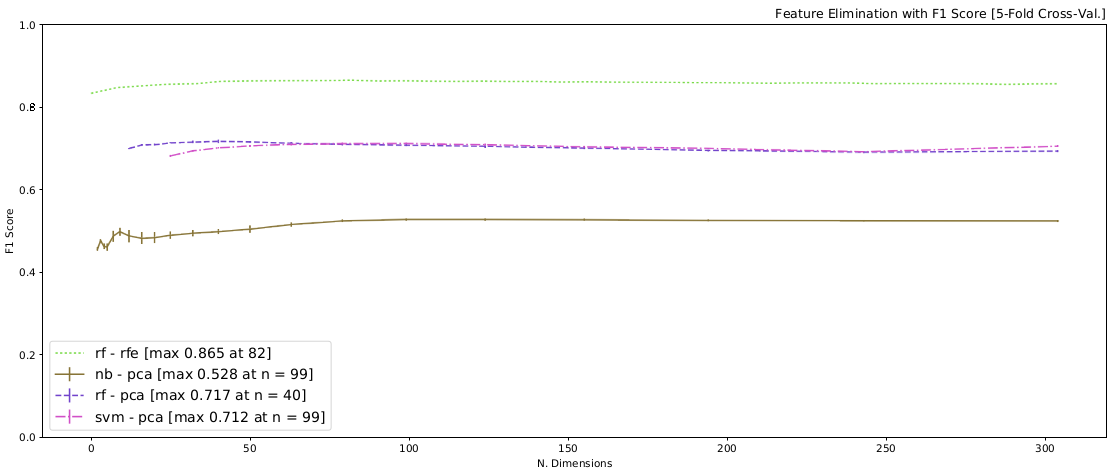
\includegraphics[width=0.9\textwidth]{feat_elim}
                \caption{$F_{1}$ Score as dimensionality is varied using Recursive Feature Elimination and Principal Component Analysis.}
                \label{fig:exp-clf-opt-featsel-grph}
            \end{figure}
            \begin{wraptable}{r}{0.3\textwidth}
                \scriptsize
                \singlespacing
                \centering
                    \begin{tabular}{ |l||c|c| } 
                        \hline
                        Classifier & N. PCA & N. RFE \\ 
                        \hline
                        \hline
                        NB & 99 & \xmark \\
                        RF & 40 & 88 \\
                        SVM & 75 & \xmark\\
                        \hline
                    \end{tabular}
                \caption{Optimal Feature-Space Dimensional Reduction Values}
                \label{fig:exp-clf-opt-featsel-elim}
            \end{wraptable}
            
            Feature selection will be performed in three stages. Firstly, we apply two methods of cross-validated feature elimination: principal component analysis, \code{PCA}, with truncation; and recursive feature elimination, \code{RFE}. With current implementations, only the random forest classifier is able to recursively eliminate features, this is reasoned in \ref{subsec:pl-test-stan}. Figure \ref{fig:exp-clf-opt-featsel-grph} shows $F_{1}$ scores as the number of dimensions are truncated, for RFE the reduction is carried out in linear steps due to implementation limitations; for PCA the scale is exponential, beginning from the number of features and reducing by a factor until there are only a small number of features left, with the features determined as least informative being removed first. The exponential scale reflects the expectation that the total collection of features contain high degree of redundant information, implying there will be more significant effect on performance at lower dimensions. Similar plots for the other performance metrics are also generated. The degree of dimensional reduction determined most optimal is shown in table \ref{fig:exp-clf-opt-featsel-elim} with consideration of all discussed metrics; some results with a high $F_{1}$ score also suffer from highly skewed predictions where the true positive rate may be very high but the true negative rate is less than a half.
            % \begin{wraptable}{l}{0.7\textwidth}
            %     \scriptsize
            %     \singlespacing
            %     \centering
            %         \begin{tabular}{ |l||c|c|c|c|c|c| } 
            %             \hline
            %             Classifier & Features & $F_{1}$ & AUC-ROC & AUC-PR & TPR & TNR \\ 
            %             \hline
            %             \hline
            %             NB & \code{MFCC}$\in\mathbb{R}^{13}$ & $0.601$ & $0.843$ & $0.626$ & $0.634$& $0.864$ \\
            %             \hline
            %             RF & \code{RFE}$\in\mathbb{R}^{88}$ & $0.710$ & $0.920$ & $0.800$ & $0.676$ & $0.934$\\
            %             \hline
            %             SVM &\code{RFE}$\in \mathbb{R}^{88}$& \boldmath$0.745$ & \boldmath$0.928$ & \boldmath$0.831$ & \boldmath$0.728$& \boldmath$0.935$ \\
            %             \hline
            %         \end{tabular}
            %     \caption{Results of feature selection.}
            %     \label{tbl:exp-clf-opt-feat-res}
            % \end{wraptable}
            
            The second stage is feature selection. For each classifier, we cross-validate performance over the following configurations: each feature in isolation; all the features combined; the optimal \code{PCA}-reduced feature set, specific to each classifier; and the the \code{RFE}-reduced feature set, as determined by the random forest. The best performing configuration is then tested on the held-out set. Again it is emphasised that no decisions are made based on test-set evaluations, only on cross-validation performance; they are included as an informative view on the progression of optimisation.
            
            %Granitto2006 - original RF-RFE
            %Guyon2002 - original SVM-RFE, more traditiona
            There is scope for use of other feature selection algorithms including SVM-RFE, Mean-Squared-Error (MSE) linear discriminant, and Fisher linear discriminant (LDA) \cite{Guyon2002}; but time has not been devoted to implementing these as they are unlikely to lead to any significant performance improvements over the features selected already.
            
            % \begin{wraptable}{r}{0.73\textwidth}
            %     \scriptsize
            %     \singlespacing
            %     \centering
            %         \begin{tabular}{ |l||c|c||c|c|c|c|c| } 
            %             \hline
            %             Classifier & \code{winlen} & \code{winstep} & $F_{1}$ & AUC-ROC & AUC-PR & TPR & TNR \\ 
            %             \hline
            %             \hline
            %             NB      &$0.089$&$0.0445$&$0.642$&$0.873$&$0.680$&$0.636$&$0.901$\\
            %             \hline
            %             RF      &$0.058$&$0.029$ &$0.759$&$0.942$&$0.847$&$0.728$&$0.945$\\
            %             \hline
            %             SVM     &$0.058$&$0.029$ &\boldmath$0.793$&\boldmath$0.951$&\boldmath$0.873$&\boldmath$0.769$&\boldmath$0.951$\\
            %             \hline
            %         \end{tabular}
            %     \caption{Results of varying window length and step size.}
            %     \label{tbl:exp-clf-opt-feat-win}
            % \end{wraptable}
            
            Features generated in this section are generated from windowed sections of the raw signal. If the windows are too small, sufficient information from the signal may not be captured; if the windows are too large then temporal resolution will be poor. The length and overlap of the windows are determined by the parameters \code{winlen} and \code{winstep} that default to $0.025$ and $0.01$ respectively, discussed in more detail in section \ref{subsec:pl-feats-software}. Constraints on these parameters are 
            \begin{align}
                \text{winstep} < \text{winlen, winstep} > \frac{1}{\text{fs}} \text{, and winlen} < \text{siglen}.
            \end{align}
            Millions of permutations of these parameters are possible; to restrict the domain further, the semi-arbitrary\footnote{Many time-windowing algorithms use this constraint by default \cite{MathWorks,Octave}.} constraint \code{winstep}$=$\code{winlen}$/2$ will be imposed. For the traditional classifiers used in this report, better performance is expected with smaller windows; there will be more samples for training that will capture more high-frequency details of the signal. A convolutional neural network (CNN), however, may perform better over larger windows with less overlap \cite{Han} due to the way the inputs are filtered over. Exponential spacing will be used for the window lengths to reflect the expectation of better performance for smaller resolutions, with the window size reducing from \SI{32}{\milli\second} to \SI{1}{\milli\second}. Figure \ref{fig:exp-clf-opt-svmfeatwin} shows a box plot of $F_{1}$ scores over the five folds of SVM validation; as the window sizes increase, the variance of the results increase dramatically as less samples are available and predictions are influenced more by outliers. 
            
            \begin{figure}[ht]
                \centering
                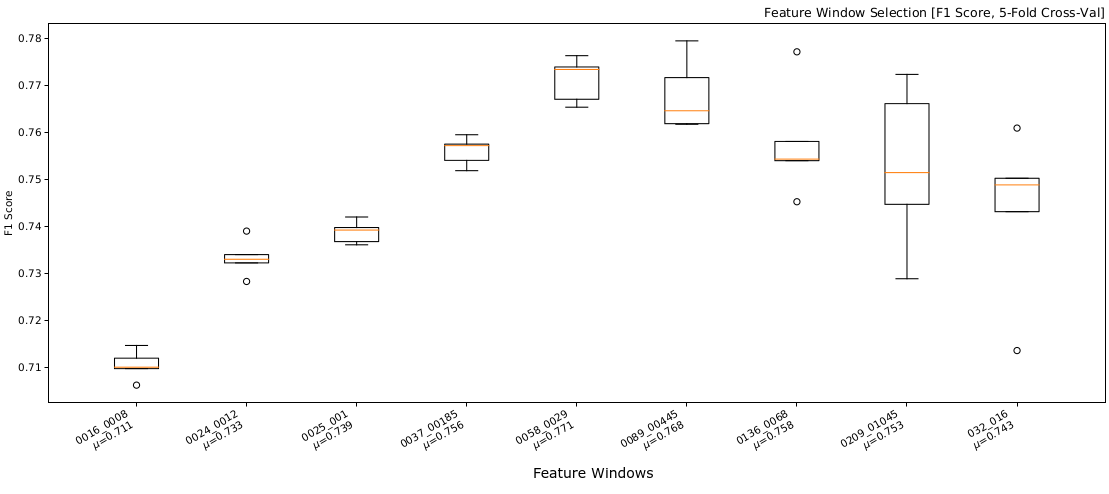
\includegraphics[width=0.9\textwidth]{svm_featwin}
                \caption{$F_{1}$ scores as window length and overlap is varied.}
                \label{fig:exp-clf-opt-svmfeatwin}
            \end{figure}
  
        
        \subsubsection{Classifier Hyperparameters}
        \label{subsubsec:exp-clf-opt-param}
            Subsequent to selection of optimal features, classifier hyperparameters are determined. Computational load reduction due to the partial feature set allows a more comprehensive grid search of parameters to be carried out. Cross-validated grid search will be applied over the random forest and SVM classifiers; the naive Bayes implementation only has the option to vary class priors which should be determined from the data.
            
            \begin{figure}[ht]
                \centering
                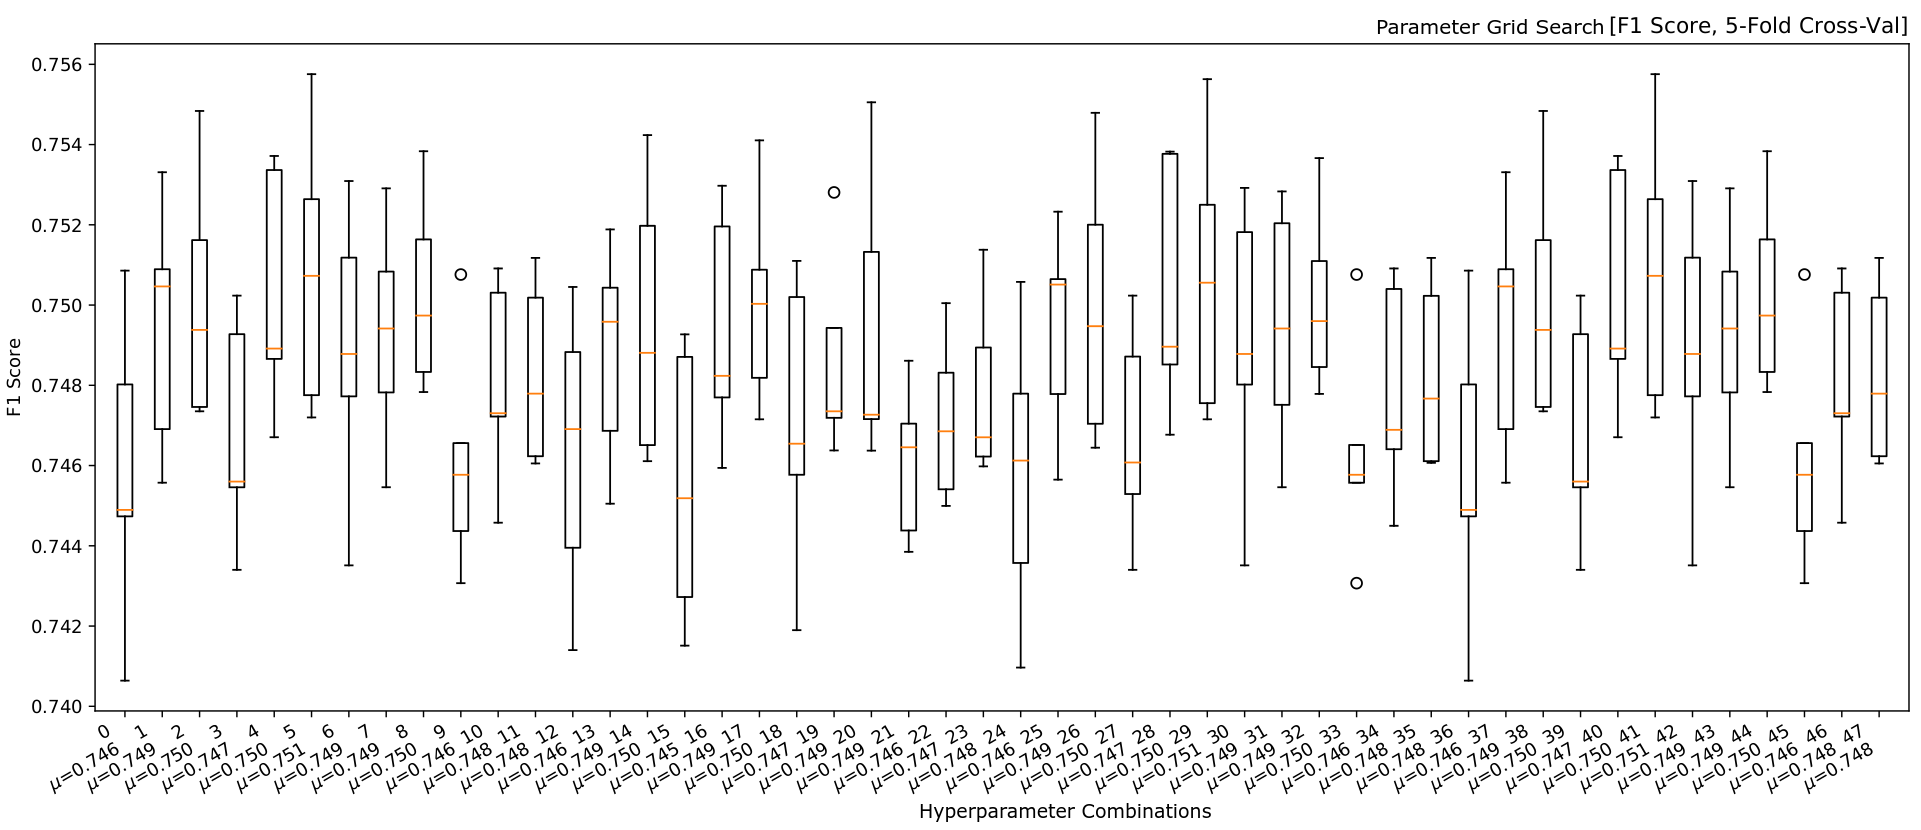
\includegraphics[width=0.9\textwidth]{hyperparameter_xval}
                \caption{$F_{1}$ scores as random forest hyperparameter combinations are cross-validated.}
                \label{fig:exp-clf-opt-hyp}
            \end{figure}
            
            Cross-validated grid search over the classifier hyperparameters must first be done \textit{very} coarsely, then refined in areas where performance is promising. For example, the \code{'max\_features'} parameter, describing the number of features to consider when splitting samples at a node of a random forest, can take an integer anywhere between $1$ and the dimension of the feature matrix, $X_{10} \in \mathbb{R}^{304}$; many of these parameters exist so combinations can reach into the millions. Grid search is executed three times over the random forest and twice over the SVM, where each iteration refines the bounds of the search. Results show straying from default parameters, which often involved restricting a previously unbound value, such as \code{'max\_depth'} of the random forest, negated performance. An example cross-validated hyperparameter search output is shown in figure \ref{fig:exp-clf-opt-hyp}, where the experiment is the second grid-search over the random forest. On the $x$ axis lies each possible combination of hyperparameters in the defined grid, where the number corresponds to a particular combination. There are clear trends within the data corresponding to particularly influential parameters such as \code{'n\_estimators'}, which is the only parameter to be updated in this section; the rest remain unchanged for both the random forest and the SVM. 
            
            % In the first round, the classifier is trained/tested $192$ times for each fold. Results show that increasing any of the parameters \code{max\_samples\_split}, \code{min\_samples\_leaf}, \code{max\_leaf\_nodes} resulted in poor metrics; these will be left at default. Use of the decision criterion \code{"entropy"} showed consistently better performance over \code{"gini"}. The rest of the hyperparameters had more subtle effects so they are searched over a more comprehensive space. 
            % \twN{More details on parameters - provide in implementation section}
            
            
            % Figure \ref{fig:exp-clf-opt-hyp} shows the cross-validation results; where each number corresponds to a particular configuration. The best performing configurations have the highest number of trees, $300$. Setting \code{max\_depth} only reduces performance, whereas tuning \code{max\_features} to a value around $60$ improves over the default value of $\sqrt{ \text{N}_{Features}}=9$. The final fine-grained cross-validation done over the number of trees and \code{max\_features} ensures the best performance is reached, results of which are presented in table REF; details of parameter grids are located at the end of this section in table REF.        
            
            % SVM: gridsearch over C and gamma showed that c=10, gamma=auto (1/nfeats) provided best performance, shrinking off massively faster convergence
   

        \subsubsection{Class Balancing}
        \label{subsubsec:exp-clf-opt-class}
            Subsequent from this section, cross-validation will be over ten folds, increasing from five due to the smaller number of parameters that need to be found and the decreased training times from reduced feature dimensions. Cross-validated tests show that balancing classes results in marginally improved performance for the naive Bayes classifier and marginally reduced performance for the SVM and random forest in terms of the $F_{1}$ score. True positive and true negative rates are influenced by the training data class proportions; training on a higher proportion of non-mosquito signals will result in a less sensitive classifier. To maximise generalisability of the classifier, classes in the training data should equally represented. This experiment reveals the reduction of samples for class-balancing does not significantly hinder classifier performance and allows a classifier to be trained with minimal bias from the proportions of the training data. Should the reduction of samples significantly affect performance, then weightings could be applied to training samples, with the over-represented class having a reduced influence over the classification decision. Many techniques exist for learning from imbalanced data, random undersampling is sufficient for this particular problem; more advanced techniques are summarised by \textcite{He2009}.
            % Table \ref{fig:exp-clf-opt-class-res} shows how balancing the training data can affect the results.
            % \begin{wraptable}{r}{0.45\textwidth}
            %     \scriptsize
            %     \singlespacing
            %     \centering
            %         \begin{tabular}{ |l|c|c|c|c| } 
            %             \hline
            %             Classifier & $F_{1}$ & ROC Area & TPR & TNR \\ 
            %             \hline
            %             \hline
            %             NB          & $0.$ & $0.$  & $0.$ & $0.$\\
            %             NB balanced & $0.$ & $0.$ & $0.$ & $0.$\\
            %             \hline
            %             RF          & $0.$ & $0.$ & $0.$ & $0.$\\
            %             RF balanced & $0.$ & $0.$ & $0.$ & $0.$\\
            %             \hline
            %             SVM          & $0.$ & $0.$ & $0.$ & $0.$\\
            %             SVM balanced & $0.$ & $0.$ & $0.$ & $0.$\\
            %             \hline
                    
            %         \end{tabular}
            %     \caption{Results of testing balanced training data against non-balanced training data.}
            %     \label{fig:exp-clf-opt-class-res}
            % \end{wraptable}
            % In all three cases, classifiers with balanced training data outperform those with imbalanced training data. 
            
            % Although overall performance is better, it is interesting to note how balancing classes skews the TPR and TNR to, rather intuitively, increase the former and decrease the latter; a potential technique to tune the classifier at later stages. Further experiments will balance the training data to maximise performance.
        
        \subsubsection{Audio Normalisation}
        \label{subsubsec:exp-clf-opt-normaud}
            % \begin{wraptable}{r}{0.7\textwidth}
            %     \scriptsize
            %     \singlespacing
            %     \centering
            %         \begin{tabular}{ |l||c|c|c|c|c|c|c| } 
            %             \hline
            %             Classifier & \specialcell{Audio\\Normalised} & $F_{1}$ & AUC-ROC & AUC-PR & TPR & TNR \\ 
            %             \hline
            %             \hline
            %             NB      &\checkmark &$0.642$&$0.873$&$0.680$&$0.636$&$0.901$\\
            %             NB      &\xmark     &$0.684$&$0.906$&$0.733$&$0.730$&$0.884$\\
            %             \hline
            %         \end{tabular}
            %     \caption{Comparing predictive performance with and without audio normalisation.}
            %     \label{tbl:exp-clf-opt-normaud-res}
            % \end{wraptable}
            Running cross-validated tests over features generated from audio signals with combinations of \code{'zero-mean'} and \code{'unit-var'} applied shows that predictions made by both the random forest and and SVM classifiers are unaffected by audio normalisation; the naive Bayes classifier, however, performs better without any audio normalisation. The audio signals will continue not being normalised, circumventing the issues discussed in \ref{subsubsec:exp-clf-ass-aud}.
        \subsubsection{Label Selection}
        \label{subsubsec:exp-clf-opt-label}
            For each classifier, all selected label aggregation policies in tables \ref{tbl:exp-clf-known-tstlbls-bintbl} and \ref{tbl:exp-clf-known-tstlbls-multitbl} are tested. For the multi-class labelling scheme, the `one vs. rest' transformation strategy is tested as well as the classifiers native multi-class implementation for the random forest and SVM classifiers. Top performing combinations are chosen based on cross-validation tests. Multi-class label aggregation provides the best performance across all three classifiers. Although, increase of prediction quality for the SVM only marginal and at the cost of 5\% rejection of predictions and increased computing time, so the \code{'conf'} labelling scheme is kept in place.

    \subsection{Summary}
    \label{subsec:exp-clf-summary}
        In this section, three classifiers have been chosen and optimised from baseline configurations and assumptions. The naive Bayes classifier improves with respect to every performance metric. The random forest drops in $F_{1}$ score from the base configuration but becomes a more balanced classifier with improved AUC values. Marginal improvements are seen over the SVMs performance metrics. Both the random forest and SVM now use a multi-class labelling scheme, rejecting uncertain outputs. This results in a $\sim5\%$ loss of output predictions which manifests as shown in figure \ref{fig:exp-clf-summary-rej}, where the outputs have been rejected in the presence of noise.
        \begin{figure}[ht]
            \centering
            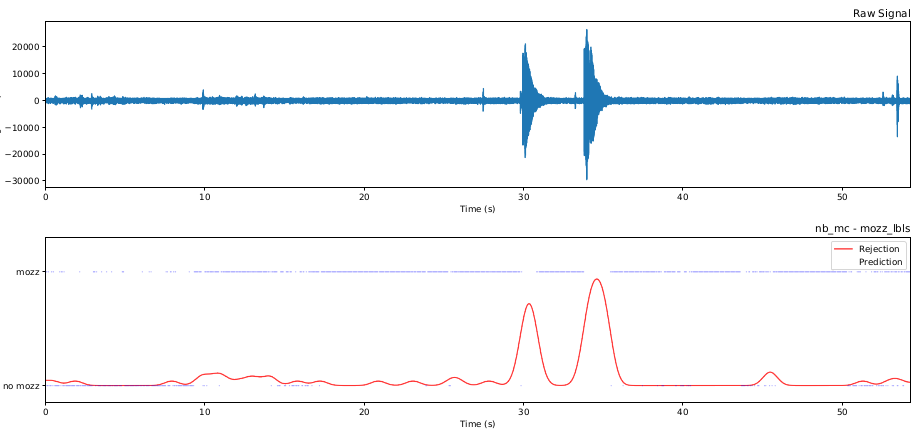
\includegraphics[width=0.9\textwidth]{rejection}
            \caption{Output from a naive Bayes classifier using a multi-class labelling scheme and rejecting predictions that fall in class $2$, corresponding to two people agreeing there is a mosquito present and two disagreeing.}
            \label{fig:exp-clf-summary-rej}
        \end{figure}
        Further optimisations could be carried out over this pipeline by including the previously disregarded classifiers as well as trying an iterative approach in which the diagram in figure \ref{fig:exp-clf-overview-opt} would be looped back to the start, using the parameters found through optimisation, and iterated until convergence. This could be used in unison with random seeding of parameters to ensure local minima are avoided. This is left outside of the report to focus on post-processing that can further improve classification performance and ultimately mosquito detection.